\documentclass{article}

\usepackage{booktabs}
\usepackage{multirow}
\usepackage{amsmath}
\usepackage{hyperref}
\usepackage{overpic}
\usepackage{amssymb}

\usepackage[accepted]{dlai2022}

%%% STUDENTS: FILL IN WITH YOUR OWN INFORMATION
\dlaititlerunning{DLAI Project: World Models in MiniGrid}

\begin{document}

\twocolumn[
%%% STUDENTS: FILL IN WITH YOUR OWN INFORMATION
\dlaititle{DLAI Project: World Models in MiniGrid}

\begin{center}\today\end{center}

\begin{dlaiauthorlist}
%%% STUDENTS: FILL IN WITH YOUR OWN INFORMATION
\dlaiauthor{Dennis Rotondi 1834864}{}
% \dlaiauthor{Donato Crisostomi}{}
% \dlaiauthor{Emanuele Rodolà}{}
\end{dlaiauthorlist}

%%% STUDENTS: FILL IN WITH YOUR OWN INFORMATION
\dlaicorrespondingauthor{Dennis Rotondi}{rotondi.1834864@studenti.uniroma1.it}

\vskip 0.3in
]

\printAffiliationsAndNotice{}

\begin{abstract}
%
In this report are presented reasoning and investigations to complete the project 06.
\href{https://github.com/DennisRotondi/dlai_project}{Code here.}

\end{abstract}

\section{Introduction}
Sequential decision making, commonly formalized as Markov Decision Process (MDP) optimization, is a key challenge in artificial intelligence. Two successful approaches to solve this problem are planning
and reinforcement learning. These may actually
be combined, in a field which is known as model-based reinforcement learning; for which a definition is: "any MDP approach that $i)$ uses a model (known or learned) and $ii)$
uses learning to approximate a global value or policy function" \cite{mb_survey}.
It's important to notice that the only engagement of a deep learning architecture does not make an algorithm model based, indeed in 
traditional RL (model-free RL) small networks are used to improve the learned policy through trial and error, but due to the bottleneck of credit assignment problem, i.e. figuring out which steps caused the resulting feedback or which should be blamed for the final result, it's hard to handle
NNs with million of parameters as predictive structure. Instead in MBRL it's all about the anology that to handle the vast amount of information that flows through our daily lives, our brain learns an abstract representation of both spatial and temporal aspects of this information \cite{brain_article}, thus large structures are not only possible but also encouraged.%:  World models are an explicit
% way to represent an agent's knowledge about its environment in a parametric model that can make predictions about the future.
\section{Related Work}
Model Based RL is not an invention of the new millennium, many 
research papers yet in '90s were discussing and analyzing the different RL branches \cite{Atkeson97acomparison}.
 However it's with the recent explosion of deep learning  
%  also thanks to the outstanding frameworks developed and modern GPU accelerators of the last years 
 that new progresses have been achieved, a line of the new era can be delimited by the nice World Model work 
 \cite{wm}: 
%  in what follow
 we'll focus on this generation of algorithms. 
 To solve the Car Racing and VizDoom scenario, here the authors built three NNs: one to learn the environment, one to memorize and predict the next observation and one to control the agent. 
 On this skeleton google research realized and published different models to master the Atari games: SimPLe \cite{simple}, where
 a policy is deployed to collect more data in the original game, achieving SOTA in sample-efficiency at that time; DreamerV2 \cite{dreamerv2} builds upon the Recurrent State-Space Model also used in PlaNet \cite{planet} and DreamerV1 \cite{dreamerv1}, each visual observation into a 32 distributions over 32 classes, the meanings of which are determined automatically as the world model learns: it achieves human-level performance! 
\section{Method}
% For the pythonic part of the project 
I've decided to reproduce the structure of the reference paper suggested applied to the 
the Minigrid gym \cite{gym_minigrid}, a very simple grid-based env which has the pro of having many variants, I've focused on the obstacle grid to build the training set. This toy problem has been 
chosen maily for practical reasons: due to limited hardware I cannot train using 200M samples like Dreamer who uses the google servers, then my main objective is to investigate how this solution works 
while doing practice with the course tools at my best. For the sake of completeness I've also tried more complex gyms,
%  like the Atari and Procgen ones, 
but what prevents to reach high performance is, like experienced by the google team, the object vanishing problem: crucial aspects of the world (enemies to kill, the agent etc.) are not captured by the vision structure, 
but what's this vision system?  
\subsection{Variational Autoencoder}
The vision model is a Variational Autoencoder which embed the 3D 64x64x3 image observation into a 1D lower dimension latent vector $z_t$. It does not only learn how to reconstruct the input but also to compress the training distribution into $N_0,_I$ using the KLD loss term. 
The best training results are thanks to Adam optimizer and a starting LR: 1e-3, a WD: 1e-5 and a Beta: 0.01 factor to balance KLD term and the MSE reconstruction loss. Moreover, to reduce the generalization error Earlystopping and ReduceLROnPlateau techniques have been employed.
\begin{figure}[h!]
    \centerline{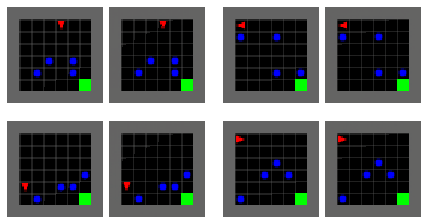
\includegraphics[scale=0.5]{./imgs/vae_results.png}}
    \caption{\label{baseline}
    Result of the VAE training: on the right recon. images.}
    \label{fig:vae}
\end{figure}
\subsection{MDN-RNN}
The second network has the role of memory and to predict the future (next state and termination condition). It consist in an LSTM \cite{lstm} which output is processed by a Mixture Density Network \cite{mdn}. 
LSTM is a particular RNN developed to overcome the vanishing gradient problem, the general idea is  is that it takes as input a sequence of vectors $x_1, ..., x_n$ and an initial state vector $h_0$ and it returns a list of hidden state vectors $h_1, ..., h_n$ and a list of output vectors $\hat{y}_1, ..., \hat{y}_n$ where each $\hat{y}_i$ is a function of the corresponding state vector $h_i$: a kind of memory of the previous $i$ inputs; a constant error flow within special cells and access to the cells is handled by multiplicative gate units.
To not overfit the next state prediction into a sigle $z_{t+1}$ MDN will predict a class of probability distributions called Gaussian Mixture Models, where the output value is modelled as a weighted sum of multiple Gaussians, each with different means and stds.
The general training setup is similar to vae's one, the difference is in the training loss: part is a MSE on for done state
%  (can be seen as a classification problem where 0 means the episode will not end and 1 the opposite) 
 and part is the log-likelihood of the gmm eq~\ref{eq:mdn_loss}: K is the number of gaussians, $\Pi_k$, $\phi_k $, $\mu_k$, $\sigma_k$ the weight, distribution, mean and std for gaussian k.
\begin{equation}\label{eq:mdn_loss}
loss(y | x) = -log[ \sum_{k}^{K} \Pi_{k}(x) \phi(y, \mu_{k}(x), \sigma_{k}(x))]
\end{equation}
The big drawback of this loss is that is not lower bounded since the mixture components may collapse in a data point making the loss decrease to arbitrarily small values.
\subsection{Controller}
Eventually who's responsible to choose the action, given the latent embedding of the observation and the hidden prediction, is a simple MLP to leave all the model complexity to the vision and memory.
Learning controller's parameters for this task is a difficult non-linear non-convex black-box optimization problem, where the CMA-ES \cite{cmaes} is know to work well.
It is an algorithm that can take the results of each generation, and adaptively increase or decrease the search space for the next generation around a variance parameter sigma: 100.
The learning procedure is based on an ask-tell interface, where the solver initially guess some possible set of parameters, then rollouts are performed and rewards for each set given back to the solver.
\section{Results}
I've decided to test the performances also in simpler variants of the MiniGrid: empty (no obstacles), random (empty + random start). 
Results are summarized in table~\ref{tab:results}, average of 1000 rollouts reward is between [-1, 0.96].
Training only the controller in the empty world will solve easily the task receiving every time the highest possible reward. 
% Using this learned policy in the obstacle world it's possible to notice that the agent see the obstacles and in a certain sense tries to avoid them, but it's never able to win. 
Almost the same apply for the random empty grid, here we always win but not always with the shortest path, my guess is that since the
lstm is initialized always with the same hidden states, it needs some steps to figure out where it is and predict the right state.
In the obstacle grid,
% , the core of this experiment and the hardest one, 
% if we do not penalize the "non moving from square behavior" the policy will be to stay in the starting position 
% % until the limit steps are reached 
% (so the average reward is 0), if we penalize it 
the optimal policy, that wins in the $20\%$ of the cases is the same of empty grid: the upper rightmost square is reached by the agent, then it turn right and go straight to the green gol square.  


\begin{table}[h!]
    \caption{Trained on (row) vs Tested on (col)}
    \label{tab:results}
    \begin{center}
    \begin{small}
    \begin{tabular}{p{0.16\linewidth} | ccccc}
    \toprule
    & empty & random & obstacles \\
    \midrule
    empty      & 0.96 & 0.22 & -0.93 \\
    random     & 0.91 & 0.88 & -0.98 \\
    obstacles     & 0.96 & 0.16 & -0.66 \\
    \bottomrule
    \end{tabular}
    \end{small}
    \end{center}
    \vspace{-0.5cm}
\end{table}

\section{Discussion and conclusions}
% Recent advances in deep RL have enabled model-based approaches 
% to learn accurate world models from image inputs, this can be a shortcut to
%  since 
World models facilitate generalization and can predict the outcomes of 
potential actions to produce faster good policies. Learning with statistical uncertainty in the virtual environment make the final policy more robust
as shown in~\cite{wm} for the VizDoom game, there the score attained in the real environment was much higher than the one obtained inside the dream.
But being in a dream has not only positive sides: inevitably we introduce sources of approximation error
that could be converted into quibble that allows the agent to cheat: for example some position where enemies cannot hit him; this implies to take into account a problem not present in the original environment.
Possible evolutions of this paradigm are the unification of the structure, so that running an action at the end of the pipeline
take a role in the learning process of the agglomerate, one could also try to replace VAE and MDN-RNN with higher capacity models like Transformers \cite{transformers}. Extending the latent space as done by \cite{dreamerv2} is the key to reduce the
object vanishing problem, furthermore google ai sees world models that leverage large offline datasets, long-term memory, hierarchical planning, and directed exploration.\\
% Completing this homework has been a full journey into the deep learning field: 
% I started from making the dataset, passing through the creation and training 
% of three different neural networks using the standard approach and a more 
% complex one required by the non-convexity of the problem; this while exploiting 
% many of the most recent and sophisticated tools in the life of a machine learning scientist.

% \newpage
\bibliography{references.bib}
\bibliographystyle{dlai2022}

\end{document}